\chapter{Multi-Robot Target Localization}


\section*{Problem Description}

Multi-robot target localization involves a team of robots collaboratively estimating the positions of one or more targets based on noisy
 sensor measurements. In this scenario a team of robots, each equipped with sensors for detecting targets within a limited sensing range, 
 and these measurements are corrupted by noise. 
The goal is to design and implement a distributed strategy that enables the robots to cooperatively locate the targets and improve the accuracy 
of the estimation compared to individual measurements.


For visualization of the context, in general, we have the following.
\begin{figure}[h]
    \centering
    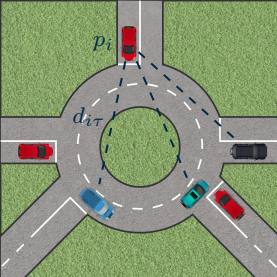
\includegraphics[width=0.4\textwidth]{img/Cap1/multi_robot_localization.png}
    \caption{Example of multi-robot target localization problem. A team of robots observing multiple targets. Noisy measurements are represented with dashed lines.}
    \label{fig:multi_robot_localization}
\end{figure}

where we have a $N \in N $ robots that estimate the positions of multiple unknown targets in a cooperative mode, using only local, noisy distance measurements. 
Each robot is assumed to be aware only of its own position and of the distances (corrupted by noise) to nearby targets, and can exchange information solely with 
its neighbors in a communication graph.


To tackle this challenge, the problem is approached in two stages:
\begin{itemize}
    \item \textbf{Task 1.1 - Distributed Consensus Optimization}: this focuses on the implementation and analysis of a distributed consensus optimization algorithm Gradient Tracking
     which allows robots to collaboratively minimize a global objective function.
    \item \textbf{Task 1.2 - Cooperative Multi-Robot Target Localization}: this builds an algorithm to solve the specific localization problem, defining suitable cost functions that
     encode the discrepancy between the measured distances and the estimated positions of the targets.
\end{itemize}

The proposed solution must be robust, scalable, and efficient, capable of handling different communication topologies and noisy sensor data, while guaranteeing convergence of the 
estimates across the network.

\subsection*{Code Structure Note}

For the sake of modularity and clarity, the implementation has been organized into multiple files, each responsible for a specific aspect of the project. The code is organized as 
follows:

\begin{itemize}
    \item \texttt{utils\_graph.py}: File that contains utility functions for generating and handling different graph topologies (e.g., cycle, path, star,erdos\_renyi) and computing 
    Metropolis-Hastings weights.
    \item \texttt{utils\_world\_generation.py}: File for creating the simulated environment, including the generation of agents and targets within a bounded space.
    \item \texttt{gradient\_tracking.py}: File to implementation of the Gradient Tracking algorithm used in both tasks, with same different.
    \item \texttt{cost\_functions.py}: Definition of the local and global cost functions used in the optimization problem.
    \item \texttt{utils\_visualization.py}: File dedicated to plotting the evolution of the cost function and gradients, and optionally animating robot movements.
    \item \texttt{main.py}: Entry point of the simulations, used to set parameters and run both tasks.
\end{itemize}

This modular structure enables the reuse of core components and makes the transition from consensus optimization (Task 1.1) to cooperative target localization (Task 1.2) seamless.



\section{Distributed Consensus Optimization}

\subsection{Problem Statement}
In this task, we address a distributed consensus optimization problem arising in multi-agent systems. The objective is to solve an unconstrained optimization problem of the form:

\begin{equation}
    \min_{z \in \mathbb{R}^d} \sum_{i=1}^N \ell_i(z),
\end{equation}
where:
\begin{itemize}
    \item \( z \in \mathbb{R}^d \) is the global decision variable to be optimized,
    \item \( N \in \mathbb{N} \) is the number of agents (robots),
    \item \( \ell_i: \mathbb{R}^d \rightarrow \mathbb{R} \) is a local objective function known only to agent \( i \).
\end{itemize}

Each agent \( i \) has access only to its own cost function \( \ell_i(z) \) and can communicate with a limited set of neighboring agents defined by a communication graph 
\( \mathcal{G} = (\mathcal{I}, {E}) \), where \( \mathcal{I} = \{1, \dots, N\} \) is the set of nodes and \( E \subseteq \mathcal{I} \times \mathcal{I} \) is the set of edges. 

\noindent
The goal is to design a distributed algorithm that allows all agents to cooperatively find a minimizer of the global cost function by exchanging information only with their 
immediate neighbors in the graph \( \mathcal{G} \).
\noindent
To evaluate the performance of the distributed consensus optimization algorithm, are implemented a different simulation. In particular, consider different types of graph structures 
such as cycle, path, star, erdos\_renyi graphs to model the communication network among the agents. 

\noindent For each topology, the communication weights are defined using the \textit{Metropolis Hastings rule}, ensuring the resulting weight matrix is symmetric and doubly 
stochastic, which is essential for convergence guarantees.


\noindent In this context, consensus optimization techniques are crucial as they enable a collective decision-making process, ensuring that all agents converge to a common 
optimal solution through local computations and communications.


\subsection{Algorithm Implementation}


\begin{tcolorbox}[colback=white,colframe=black!75!black,title=ADD IMPLEMENTATION ]

\end{tcolorbox}


\section{Cooperative Multi-Robot Target Localization}

In the second part of the task, leveraging the work done in Task 1.1, the goal is to implement the \textit{Gradient Tracking} algorithm to enable a fleet of robots to cooperatively 
localize multiple targets in the environment.

\noindent
The main objective is to estimate the positions of multiple targets by using noisy distance measurements from the robots to the targets, while ensuring consensus among the robots 
on the final estimates.

\subsection{Problem Statement}
The scenario involves a set of \( N \) robots, each with an unknown position \( p_i \in \mathbb{R}^d \), and \( N_T \) static targets whose positions are to be estimated.
\noindent
Each robot obtains noisy measurements of its distances \( d_{i\tau} \in \mathbb{R}_{\geq 0} \) to each target \( \tau = 1, \ldots, N_T \). The robots aim to collectively minimize 
a local cost function defined as: 
\begin{equation}
    f_i(z) = \sum_{\tau=1}^{N_T} \left( d_{i\tau}^2 - \| z_\tau - p_i \|^2 \right)^2,
\end{equation}
    
where \( z = \mathrm{col}(z_1, \ldots, z_{N_T}) \in \mathbb{R}^{d N_T} \) is the concatenated vector of target position estimates \( z_\tau \in \mathbb{R}^d \).

By implementing the Gradient Tracking algorithm, the robots iteratively update their local estimates while exchanging information with their neighbors, achieving consensus on the 
target locations. 

\noindent
So the algorithm minimize the local cost functions cooperatively, allowing the robots to share information and iteratively update their estimates.



\subsection{Algorithm Implementation}


\begin{tcolorbox}[colback=white,colframe=black!75!black,title=ADD IMPLEMENTATION ]

\end{tcolorbox}

\section{Code Implementation}


In this section presents the implementation details of the codebase developed to solve Task 1.1 and Task 1.2. 

In particular, we distinguish the core modules, which are shared across the two tasks (e.g.utils\_graph.py, utils\_world\_generation.py, ...), and specific function that define 
the optimization problem and implement the corresponding distributed algorithm (Distributed Gradient Descent for Task 1.1 and Gradient Tracking for Task 1.2). 

What follows is an overview of the structure, key components, and how the codebase supports the objectives of each task.

\subsection{Common Utility Function and Scripts}

\subsection*{\textbf{utils\_graph.py}}
This module provides utility functions for generating and processing graphs 

\noindent Functions: 
\begin{itemize}
    \item \textbf{\texttt{ensure\_connected\_graph(G)}}: \\
    Ensures that the input graph G is connected adding an Egees between if it disconnected; 
    \item \textbf{\texttt{metropolis\_hastings\_weights(G)}}: \\
    Computes the Metropolis Hastings weight matrix $A$ for a given graph $G$. If $A$ is: 
    \begin{itemize}
        \item Not diagonal $A_{ij} = \frac{1}{(1 + max (d_i, d_j)}$ if nodes $i$ and $j$ are connected; 
        \item It is diagonal $A_{ii} = 1 - \sum_{j \not= i} A_{ij} $
    \end{itemize} 
    \item \textbf{\texttt{generate\_graph(num\_agents, type, p\_er$=$0.5)}}:\\
    \texttt{path}, \texttt{cycle}, \texttt{star}, or \texttt{erdos\_renyi}. If the generated Erdos-Renyi graph is disconnected, minimal connections are added to make it connected. 
    Returns the graph object $G$, its adjacency matrix $Adj$, and the Metropolis-Hastings weight matrix $A$.
\end{itemize}

\subsection*{\textbf{utils\_world\_generation.py}}

This module provides helper functions to generate agents and targets in a bounded $d$-dimensional environment. It also simulates noisy distance measurements within a given field of 
view (FOV)

\noindent Functions: 

\begin{itemize}
    \item \textbf{\texttt{is\_in\_fov(agent\_pos, target\_pos, radius\_fov)}}\\
    Determines whether the target is within the agent's field of view radius.

    \item \textbf{\texttt{spawn\_agent\_near\_target(target, existing\_agents, existing\_targets, world\_size, d, radius\_fov)}}\\
    Randomly spawns an agent within the FOV of a given target, avoiding overlap with existing agents and targets.

    \item \textbf{\texttt{spawn\_candidate(existing\_agents, existing\_targets, world\_size, d)}}\\
    Generates a random position in the world that does not overlap with any existing agent or target.

    \item \textbf{\texttt{generate\_agents\_and\_targets(num\_targets, ratio\_at, world\_size, d, radius\_fov)}}\\
    Creates a set of targets and agents such that each target is seen by at least 3 agents within the FOV. Additional agents are added randomly to achieve a target-agent ratio of 
    \texttt{ratio\_at}. The positions are normalized with respect to the world size.

    \item \textbf{\texttt{get\_distances(agents, targets, noise\_level, bias\_param, radius\_fov, world\_size)}}\\
    Computes both exact and noisy distances between each agent and target, limited to those within the FOV. The noise includes a uniform bias and Gaussian noise, scaled by the 
    world size.
\end{itemize}


\subsection*{gradient\_tracking\_method.py }

This module implements the \textbf{Gradient Tracking} algorithm for decentralized optimization, applicable to both localization and target estimation tasks. 
Each agent maintains and updates local estimates and gradients through message passing over a communication graph.

\begin{itemize}
\item \textbf{\texttt{gradient\_tracking\_method(agents, targets, noisy\_distances, adj, A, local\_cost\_function, alpha, max\_iters)}}:\\[2pt]
Executes the gradient tracking algorithm 
    \noindent \textbf{Algorithm steps:}
    \begin{enumerate}
        \item \textbf{Initialization:} \\
        The variable $z_0$ (local estimate) is initialized uniformly at random in $[0,1]$. Gradients $s_0$ are initialized using the local cost function.
        
        \item \textbf{Iterative updates:} For each iteration $k$:
        \begin{itemize}
            \item \emph{Estimate update:} $z^{k+1}_i$
            \item \emph{Gradient tracking update:} $s^{k+1}_i$
        \end{itemize}
        \item \textbf{Monitoring quantities:}
        \begin{itemize}
            \item \emph{Cost:} Local cost contributions summed across all agents.
            \item \emph{Gradient norm:} Norm of the global gradient estimate at each iteration.
            \item \emph{Error:} Euclidean distance between the agent's estimate $z^k_{ij}$ and the true target $j$.
        \end{itemize}
    \end{enumerate}

    \noindent \textbf{Return values:}
    \begin{itemize}
        \item $z$: Local estimates of agents over time.
        \item $cost$: Global cost function at each iteration.
        \item $norm\_grad\_cost$: Norm of the aggregated gradients.
        \item $norm\_error$: Estimation error norms for each agent-target pair over time.
    \end{itemize}
\end{itemize}

\noindent This method is suitable for both localization tasks (estimating an agent's position using anchors) and distributed target tracking (estimating moving or static targets
via multiple agents).


\subsection*{\textbf{utils\_visualization.py}}

This file contains functions to visualize the graph topology, the agents' and targets' positions in the world, and the evolution of decentralized estimation algorithms over time.

\begin{itemize}
    \item \textbf{\texttt{visualize\_graph(G)}}\\
    Draws the structure of the input graph $G$ using \texttt{networkx}.

    \item \textbf{\texttt{plot\_gradient\_tracking\_results(z, cost, norm\_grad\_cost, agents, targets, norm\_error)}}\\
    Produces a set of plots related to the gradient tracking algorithm:
    \begin{itemize}
        \item Evolution of the cost function.
        \item Norm of the gradient over iterations.
        \item Error norms for each target, shown across all agents.
    \end{itemize}
    All plots are rendered using logarithmic scale for better visualization of convergence trends.

    \item \textbf{\texttt{visualize\_world(agents, targets, world\_size, d)}}\\
    Visualizes the spatial configuration of agents and targets in 1D, 2D, or 3D space. The entities are rescaled by the world size and displayed with:
    \begin{itemize}
        \item Blue circles for agents.
        \item Red crosses for targets.
    \end{itemize}
    The function automatically adapts the axes and labels according to the dimensionality $d$.

    \item \textbf{\texttt{animate\_world\_evolution(agents, targets, z\_history, type, world\_size, d, speed=50)}}\\
    This function are usefull for the evolution of agent estimations $z$ over time using \texttt{matplotlib}'s \texttt{FuncAnimation}. It supports 1D, 2D, and 3D visualizations, and:
    \begin{itemize}
        \item Shows agents and targets as static reference points.
        \item Dynamically updates estimation points in green.
        \item Allows to visually inspect convergence of estimations to target locations.
    \end{itemize}
    The graph topology type is included in the plot title for clarity.
\end{itemize}

\subsection{Adaptation of the Method to Different Tasks}

\subsection*{\textbf{cost\_functions.py}}

The script defines two separate functions, in particular define two separated local cost functions, for each tasks, used during optimizatio. 



\begin{itemize}
    \item \textbf{\texttt{local\_cost\_function\_task1(z, p\_i, distances\_i $=$ None)}} \\
The agent seeks to estimate the target positions based only on relative displacement, without depending on any form of measurement. The cost is formulated as a weighted quadratic 
penalty on the distance between the agent's position \( p_i \) and each estimated target position \( z_j \). A positive definite matrix \( Q \) scales the contribution of each 
coordinate, and an affine term \( b \) ensures numerical stability:
    
    \[\text{cost} = \sum_{j=1}^{m} (p_i - z_j)^\top Q (p_i - z_j) + b.\]
  
    The corresponding gradient is linear, and the same for all targets, as it does not depend on any observation or measurement.

    \item \textbf{\texttt{local\_cost\_function\_task2(z, p\_i, distances\_i)}} \\
    The local cost depends on the difference between the estimated distances (based on current position estimates) and the actual noisy distance measurements received by each agent.
    The cost penalizes the squared error between measured and estimated squared distances:
    \[ \text{cost} = \sum_{j=1}^{m} \left( \| z_j - p_i \|^2 - d_{ij}^2 \right)^2. \]

    The gradient, unlike Task 1, is computed separately for each target and depends nonlinearly on both the estimated position \( z_j \) and the measured distance \( d_{ij} \). 
    This makes it more sensitive to measurement noise, but also more informative when such data is available.
\end{itemize}



\paragraph{Practical Considerations.}
Both functions return the local cost and its gradient. In Task 2, special care is taken to handle missing or undefined distance values using \texttt{np.isnan}, setting the 
corresponding gradient to zero when necessary. This ensures stability and robustness to missing data.

\subsection*{\textbf{main.py}}
The \texttt{main.py} script serves as the central entry point for the simulation, coordinating data generation, task execution, and result visualization. Its structure is 
modular and task-agnostic, making it adaptable for different estimation problems.


\begin{itemize}
    \item \textbf{Parameter Setup} \\
    The simulation settings are defined in the \texttt{PARAMETERS} dictionary, including number of targets, agent-to-target ratio, dimension of the environment, type of 
    communication graph, noise level, and field of view radius. 

    \item \textbf{Task Selection and Configuration} \\
    The script supports different tasks through the \texttt{task\_settings} dictionary, which maps each task identifier to its specific cost function and corresponding step size 
    (\( \alpha \)). The \texttt{task\_to\_run} list allows multiple tasks to be executed sequentially in a single run.

    \item \textbf{Environment and Graph Initialization} \\
    Agents and targets are randomly generated using \texttt{generate\_agents\_and\_targets()}, and their connections are defined through \texttt{generate\_graph()} according to 
    the specified topology (e.g., cycle). Distance measurements are simulated by \texttt{get\_distances()}, which produces both real and noisy measurements, subject to field-of-view 
    constraints.

    \item \textbf{Task Execution Loop} \\
    For each selected task:
    \begin{enumerate}
        \item The corresponding cost function and step size are selected.
        \item The \texttt{gradient\_tracking\_method()} is invoked to perform distributed optimization and return the full history of target estimates, costs, gradients, and errors.
        \item The resulting performance is visualized using:
        \begin{itemize}
            \item \texttt{visualize\_world()} for initial layout of agents and targets.
            \item \texttt{plot\_gradient\_tracking\_results()} for convergence diagnostics.
            \item \texttt{animate\_world\_evolution()} to display the temporal evolution of estimates.
        \end{itemize}
    \end{enumerate}

\end{itemize}
